% Preamble
\documentclass[parskip=full]{article}
\fontfamily{cmss}
% Packages
\usepackage{graphicx}
\graphicspath{{./figures/}}
\usepackage[nohead, nomarginpar, margin=2cm, foot=2cm]{geometry}
\usepackage{setspace}
\usepackage{booktabs}
\usepackage{tabularx}
\usepackage[table,x11names]{xcolor}

% Document
\singlespacing
\begin{document}
    \tableofcontents
    \pagebreak
    \section{Data intensive systems}
    \subsection{Architecture}
    The top-level architecture of the platform (Figure 1) consists of 3 microservices, with a dedicated database node for each, a command line client app and a Kafka cluster.
    The client communicates with the microservices via an HTTP API, while the microservices exchange information by sending messages to the Kafka cluster and subscribing to the required topics.
    Each microservice's data is stored in its corresponding database and is processed using the Hibernate library.

    Message exchange is implemented using the apache Kafka platform, with the flow of messages across the services divided into several topics.
    Each topic's messages are keyed with a value of the same type and messages are represented by a serializable java DTO, which are defined in the microservice publishing these messages.

    The system allows for customization and expansion of its capabilities by modifying its data exchange schema, i.e. the definitions of the various Kafka keys and values.
    The microservices can also expand their functionality by making use of parts of the message values that they are receiving but not making use of yet.
    An example of that can be seen in the trending hashtag microservice, which consumes messages from the``video-liked''topic, but is only interested in the hashtag list contained in the message value DTO. A future update of the microservice could also use the user's username from the message value to construct links between a user and their most liked hashtags, which in turn could be used to recommend videos from hashtags based on the user's interest.

    The system's architecture contributes to its fault tolerance.
    By providing a separate database node for each microservice, the system is able to continue functioning (with limited functionality) after losing one, or even two of its databases.
    Furthermore, a failure in each of the microservices does not affect the state of any others.
    The same applies to the Kafka cluster, which, after experiencing a failure in one of its nodes, will rebalance its brokers to allow for uninterrupted message flow.
    The separate databases also allow for each microservice to store the smallest possible representation of each entity.
    For example, while the video microservice could store user information such as date of birth, their posted videos and region, the subscription microservice could store only the username in order to keep track of the links between a user and a hashtag.
    This keeps the amount of exposed information to a minimum in case the security of any database container is compromised, increasing the overall security of the system.

    The microservices architecture also allows for the system to be scaled according to the users' needs.
    Each database node can handle communication with several instances of each of its corresponding microservice nodes, and more database nodes could also be created to allow for features like region-based splitting of the data to organically split the dataflow.
    For a use case like this, a load-balancing and/or container orchestration solution should be added to the system to ensure a consistent split of workload on each of the nodes.
    More Kafka nodes can also be added to the cluster to increase the capacity of the message exchange flow.

    The command line client is distributed as a JAR for the user to run on their own machine.
    The client communicates with the running system on its exposed ports and makes requests to the corresponding HTTP controllers.
    In the current version of the system, the client is not part of the docker compose cluster and communicates with it as an external connection.
    A more user-friendly approach to interacting with the system could involve the development of a front-end, which could be then added to the docker cluster and not require a java runtime to be installed on the user's machine.
    A more thorough documentation of the CLI client's capabilities is provided in section 2.1.2

    Figures 2 and 3 show a view of the system from a message exchange perspective: Figure 2 shows Kafka message keys and values, while figure 3 shows Kafka streams, consumers and producers.

    \pagebreak
    \subsection{Microservices}
    \subsubsection{Video microservice}
    The video microservice is responsible for the creation of videos, users and hashtags.
    It also allows users to interact with videos by liking, viewing or disliking them, publishing messages to the Kafka cluster when these interactions happen.
    The domain diagram of the video microservice is shown on Figure 4.

    External interactions with the video microservice are done through its 3 controllers

    \begin{itemize}
        \item VideoController - used for posting, liking, viewing and disliking videos as well as retrieving a list of all videos, with the ability to filter by hashtag name and/or author's username
        \item UsersController - used for registering new users
        \item HealthController - used for checking the overall health of the microservice - takes no parameters and returns the string``Service running''if the service is healthy
    \end{itemize}

    \subsubsection{Trending hashtag microservice}
    The trending hashtag microservice is responsible for maintaining a list of the top trending hashtags.
    The service receives data from its Kafka stream, which subscribes to the``video-liked''topic and produces``trending-hashtags''messages, which represent the number of likes associated with that hashtag over a sliding time window.
    The domain diagram of the trending hashtags microservice is shown on Figure 5.
    The duration of the sliding time window as well as the size of the leaderboard are configurable via the application properties and can be adjusted to fit customer needs (default values are 1 hour and 10 hashtags respectively).

    External interactions with the trending hashtag microservice are done through its 2 controllers:

    \begin{itemize}
        \item TrendingHashtagsController - used for retrieving the top trending hashtags.
        Since each event could be in several time windows, only records with the highest like count in the given hour were returned.
        \item HealthController
    \end{itemize}

    \subsubsection{Subscription microservice}
    The subscription microservice is responsible for tracking users' subscriptions to hashtags and providing recommended videos for a given user's subscriptions.
    The microservice uses its Kafka listeners to recreate (with minimal data) the videos, users and hashtags created in the video
microservice, adding a new relationship between users and hashtags.
The domain diagram of the subscription microservice is shown on Figure 6.
The subscription microservice mainly relies on the video microservice in terms of request validation.
It does, however, perform uniqueness checks on videos, hashtags and users, which allows it to handle out of order messages.
For example, if a message for a video being viewed arrives before a message for that same video being posted, the service will handle the discrepancy by initiating the video entity with a view count of 1 and simply no-op when handling the``video-posted''message.
This allows the subscription microservice to be more resilient to transient network failures or race conditions, where many messages concerning the same video arrive at once.

    External interactions with the trending hashtag microservice are done through its 3 controllers:

    \begin{itemize}
        \item SubscriptionsController - used to subscribe or unsubscribe to and from a given hashtag
        \item RecommendationsController - used to fetch the recommendations for a user's subscription
        \item HealthController
    \end{itemize}

    \subsubsection{Command line client}
    The command line client interacts with the microservices and provides success/error messages for POST/PUT requests.
    For GET requests returning a serialized value, the client applies a formatter to make the resulting data look presentable and easy to read.
    The client supports the following commands (a more thorough description can be found in the README in the client's code directory):

    \begin{table}
        \centering
        \begin{tabular}{|p{0.2\linewidth}|p{0.3\linewidth}|p{0.5\linewidth}|}
            \toprule
            \textbf{Command} & \textbf{Description} & \textbf{Args} \\
            \midrule
            list-videos & List all videos known to VM & -h (hashtag filter, optional), -a (author username filter, optional) \\
            post-video & Create a new video & -a (username of an existing user), -t (title of the new video), -h (list of hashtags to be added to a video, comma separated) \\
            Interact-with-video & Like, watch or dislike a video & -v (id of the video to interact with), -u (the username of an existing user who is performing the action), -t (type of interaction - LIKE, WATCH, DISLIKE) \\
            register-user & Create a new user & -u (username) \\
            list-trending-hashtags & Get the top trending hashtags &  \\
            get-recommendations & Get top videos to watch for a subscribed user & -h (name of an existing hashtag), -u (name of an existing user) \\
            manage-subscriptions & Add/remove a subscription from a user & -u (name of an existing user), -a (type of action - SUBSCRIBE, UNSUBSCRIBE), -h (name of an existing hashtag) \\
            \bottomrule
        \end{tabular}
        \caption{}
        \label{tab:cli-commands}
    \end{table}


    \pagebreak
    \subsection{Containerisation}
    The system is packaged as a docker compose cluster comprised of two yml files.
    One file consists of the definition of each microservice, its database and the Kafka cluster, while the other stores sensitive configuration data, such as database usernames and passwords.
    While such an approach is not suitable for a production environment as the secrets are stored in the same directory and are not encrypted, it acts as a proof of concept in ensuring the security of the system.

Several steps have been taken to ensure that the system does not expose unnecessary data and cannot be easily manipulated, namely the database container ports are not exposed, kafka-ui is not part of the cluster to avoid exposing message content, topic auto-creation is disabled and the adminer container is not part of the cluster.
To prevent errors relating to topics being unknown to the Kafka streams in the microservices, another Kafka container is used prior to the microservices starting.
This container, instead of running the default command, runs the``topics.sh''script, creating the necessary topics, and exits.
The wait condition for each of the microservices includes ensuring that the``topic creator''image has successfully exited.
This approach has been modified from the official Kafka streams example.
Other wait conditions for the microservices include ensuring that the service's associated database container Is healthy and that the Kafka cluster is healthy.
The microservice images also report on their own health, using their health controller.
To enable this, the``dockerBuild''task had to be modified with an extra command to ensure that the alpine base images contain the``curl''tool.
Finally, a structurizr container is part of the compose cluster, enabling an interactive high-level view of the system structure on port 3000.

Microservice and database containers are set to auto-restart on failure.
This ensures that no manual interaction with the cluster is necessary to recover from one-off failures and that the microservices are able to maintain a degree of functionality even after suffering an error.

Some steps are required to scale the cluster: while several instances of a microservice can connect to the same database without any additional configuration (simply by setting the corresponding environment variables), a load balancing solution like nginx must be used to proxy the incoming requests from the users running the CLI JAR and send them to the corresponding container.
The microservices are designed with this in mind: for example, UUID's are used for most identifiers, avoiding primary key uniqueness violations that could arise from several sequential ID generators trying to write to the database at the same time.

Having several nodes in the Kafka cluster further increases the fault tolerance of the system: in case of a failure of an individual node, the remaining nodes can simply rebalance and continue working as usual, albeit with less bandwidth.
The same applies to Kafka producers, consumers and streams within the microservices if several instances of each microservice are run simultaneously: if one such node suffers a failure, the remaining microservice nodes can rebalance and take on more partitions to consume each.

Using a container for each database as opposed to a single container for all of them has its benefits in increasing the fault tolerance too: with that approach, while a database failure would prevent the functioning of a microservice trying to read from it, other microservices will not be affected and will continue working as expected.
Furthermore, if the failed microservice will receive messages that would normally cause it to write to the database, such messages would not be processed or committed, meaning that each message will be read once the microservice returns to normal functionality.

    \pagebreak
    \subsection{Quality assurance}
    \subsubsection{Testing}
    The system has been tested using a combination of approaches to achieve the highest degree of confidence in its adherence to the requirements.
    Overall, the tests have been broken into several suites:
    \begin{itemize}
        \item Integration and unit level tests for each of the microservices
        \item Unit tests for the command line client
        \item Feature tests, interacting with the microservices through the command line and testing them working in unison
    \end{itemize}
The tests for individual microservices focused on ensuring the correct transformation between database tables and DTO's returned via each of the API's as well as the correct execution of business logic.
For each of these suites, micronaut test resources were used to spin up the required database and/or Kafka containers.
Where the test required the presence of data in the database, it  was written by injecting the repository classes provided by micronaut and creating and saving the required entities with the properties matching the requirements of the test scenario.

The test files were organized to match the package structure of each of the microservices, and tests relating to the API were grouped by the endpoint name.
To aid in readability, nested test classes have been used, annotated with @Nested.
Where class or test names were too long, @DisplayName annotations have been used to provide a clearer description of what the test aimed to achieve.

For each area of the microservices (such as API endpoints), several tests simulating both the``happy path''as well as certain edge cases were provided to ensure the system can handle unusual conditions or misshapen or missing data.
Examples of such tests included empty tables for each of the microservices, unknown identifiers and attempts to create duplicate entries in the tables where such entries would not normally be permitted.
For the trending hashtag microservice, testing involved making sure that the controller can handle overlapping time windows, which was achieved by creating entries for the same hashtag with different like counts in two overlapping time windows and then asserting that only the highest value in the last hour has been returned.

Several approaches have been taken to test the microservices' messaging capabilities: the message producers, whose implementation is handled internally by micronaut, have been tested via mocking and verifying that the correct message has been produced with the correct parameters e.g. that a``video-liked''message has been produced when a video is successfully liked (as well as verifying that no message is produced when the request fails for any reason).
Kafka consumers have been tested by injecting an instance of the consumer under test, calling its function associated with the given topic and verifying, mostly by using an injected instance of a repository, that the message has been processed correctly i.e. that the right records in the database have been created and/or updated.
Kafka streams were tested using the TopologyTestDriver class provided by apache and verified that the stream correctly transforms the messages from the input topic into messages that match the expected structure of the output topic and contain the same content.

The command line client, whose main functionality was calling the HTTP endpoints associated with each command using an injected instance of a micronaut HTTP client, was tested on an integration level by using the wiremock library to simulate the output of each microservice at the expected URL without requiring any containers to be running in the background.
Wiremock's built in verification tools have been used to ensure that each parameter is correctly interpreted by the CLI and that the necessary transformations are applied e.g. that the -h argument of the post-video command has been successfully split into individual hashtag names.
Since the CLI wrote output to the terminal, the output was captured to a ByteArrayOutputStream prior to starting each test.
This allowed the tests to ensure that the CLI can handle HTTP errors and that error responses are returned to the user.

Feature tests utilized the Testcontainers library (specifically the ComposeContainer class) to start a docker compose cluster that matched the``production''version, but provided more connections via exposing the database container's ports and providing a kafka-ui container for debugging.
Since the feature tests treated the compose container as a``black box'', creating test data via micronaut repositories was not feasible.
To overcome this, data was written directly to the tables using a SQL connection.
Utility functions were created to transform a minimal representation of entities into SQL queries.
A similar approach was used to clear the databases between tests.
The feature tests simulated typical usage, e.g. liking several videos and verifying that the trending hashtags are displayed in the correct order, with the right formatting and for the right time window.
Feature tests were moved into a separate gradle task by tagging the test classes and only including their tags when running tests under the featureTests task.

Utility functions were unit tested when applicable (i.e. when they were not simply wrappers over a getter/setter) and added to their containing microservices's test suite.

Overall, 132 tests were run, all passing, achieving 78\% class coverage and 96\% line coverage.
It should be noted that this takes the generated code, with many abstract classes, interfaces and DTO classes into account (more in section 2.2.4), which brings down the percentage of testable code.
Out of the manually written packages, the lowest coverage was achieved by the trending hashtags service at 95\% and the highest was shared by the video and subscription microservices at 99\%.

While it could be argued that using the CLI clients and/or micronaut repositories to seed test data makes the test scenarios less``pure''i.e. relies on one component of the system while testing another, the relative simplicity of the database structure and the API makes it unlikely that the clients and repositories, whose implementation is done by micronaut will cause any issues or test flakiness.

The split between integration and feature tests could be another point of criticism for the test suite.
Due to the longer startup time, longer test execution and less clarity about the insides of the microservices associated with the feature tests, they did not cover as many edge cases and relied on the lower-level tests to fill the``gaps''in coverage and business logic.
Thererfore, any suite taken on its own may not be sufficient to verify the correctness of the system.
When running them together though, the tests provide a reasonable level of coverage and ensure that the system conforms to the high-level requirements.

    \subsubsection{Addressing container vulnerabilities}
    An initial scan of the microservices' images revealed a relatively large number of high and critical vulnerabilities.
    Due to the microservices differing only slightly in terms of dependencies, the vulnerability list ended up looking very similar for all three.
    To address them, several (identical) steps were taken across each microservice:
    \begin{itemize}
        \item The base image was changed from the default (openjdk:17-alpine) to eclipse-temurin:17-alpine
        \item The``snappy-java''and``netty-handler''dependencies, whose earlier versions had known vulnerabilities, were manually upgraded in each build.gradle file to a version specified in the vulnerability's fix as described in docker scout (1.1.10.5 and 4.1.102.Final respectively)
        \item The``logback-classic''package has been upgraded to version 1.4.14 in each microservice, as specified in the suggested fix in docker scout
    \end{itemize}
Overall, these steps fixed all the detected vulnerabilities in the video and subscription microservices.
In the trending hashtag microservice, docker scout continued to pick up a single medium-tier vulnerability (CVE-2023-3511WJ), however, the description of the vulnerability suggests that it only occurs under impossible conditions and therefore does not pose a danger to the security of the trending hashtag microservice.

The initial scan of the Kafka images (bitnami/kafka:3.5) revealed a critical vulnerability in zookeeper.
Updating the image to version 3.6.1 has fixed this issue, however a single high level vulnerability remains.
Given that Eclipse jetty is the source of this vulnerability, it is likely that to fix it, one would need to change the source code that the Kafka container runs, which, is not feasible due to both the strict code reviews on apache's side and the timeframe of the project.

The mariadb image, whose containers accompany each microservice, had a critical level vulnerability coming from its outdated version of golang.
At first glance, the problem seemed like it could have simply been solved by updating go, however, a closer inspection revealed that the actual source of the vulnerability seemed to be the``gosu''tool, which itself depended on go.
At the time of writing, the latest version of gosu did not use the version of go which fixed the vulnerability.
However, the maintainers of gosu have reported a high number of false positive vulnerabilities and developed their own way of scanning for them.
With their tool, this vulnerability was not detected, therefore it could be assumed that the functioning of the microservices would not be affected by it.

Finally, the structurizr image was revealed to have 3 high severity issues, all of which related to denial-of-service attacks.
These vulnerabilities, however, were part of the underlying source code and could not be reasonably addressed in the given timeframe.
Furthermore, a failure of the structurizr container in the compose setup would not affect the actual functionality of the system in any way, with structurizr only serving an information/documentation purpose, which is duplicated in the Sirius diagrams of the microservices (See section 2.2.2)

It should be noted that medium and low vulnerabilities were investigated, but not addressed, given the limited timeframe of the project, the limited likelihood of these vulnerabilities occurring, and the low impact if they did occur.


    \section{Application of model driven engineering}
    \subsection{Metamodel}
    \begin{figure}[h]
        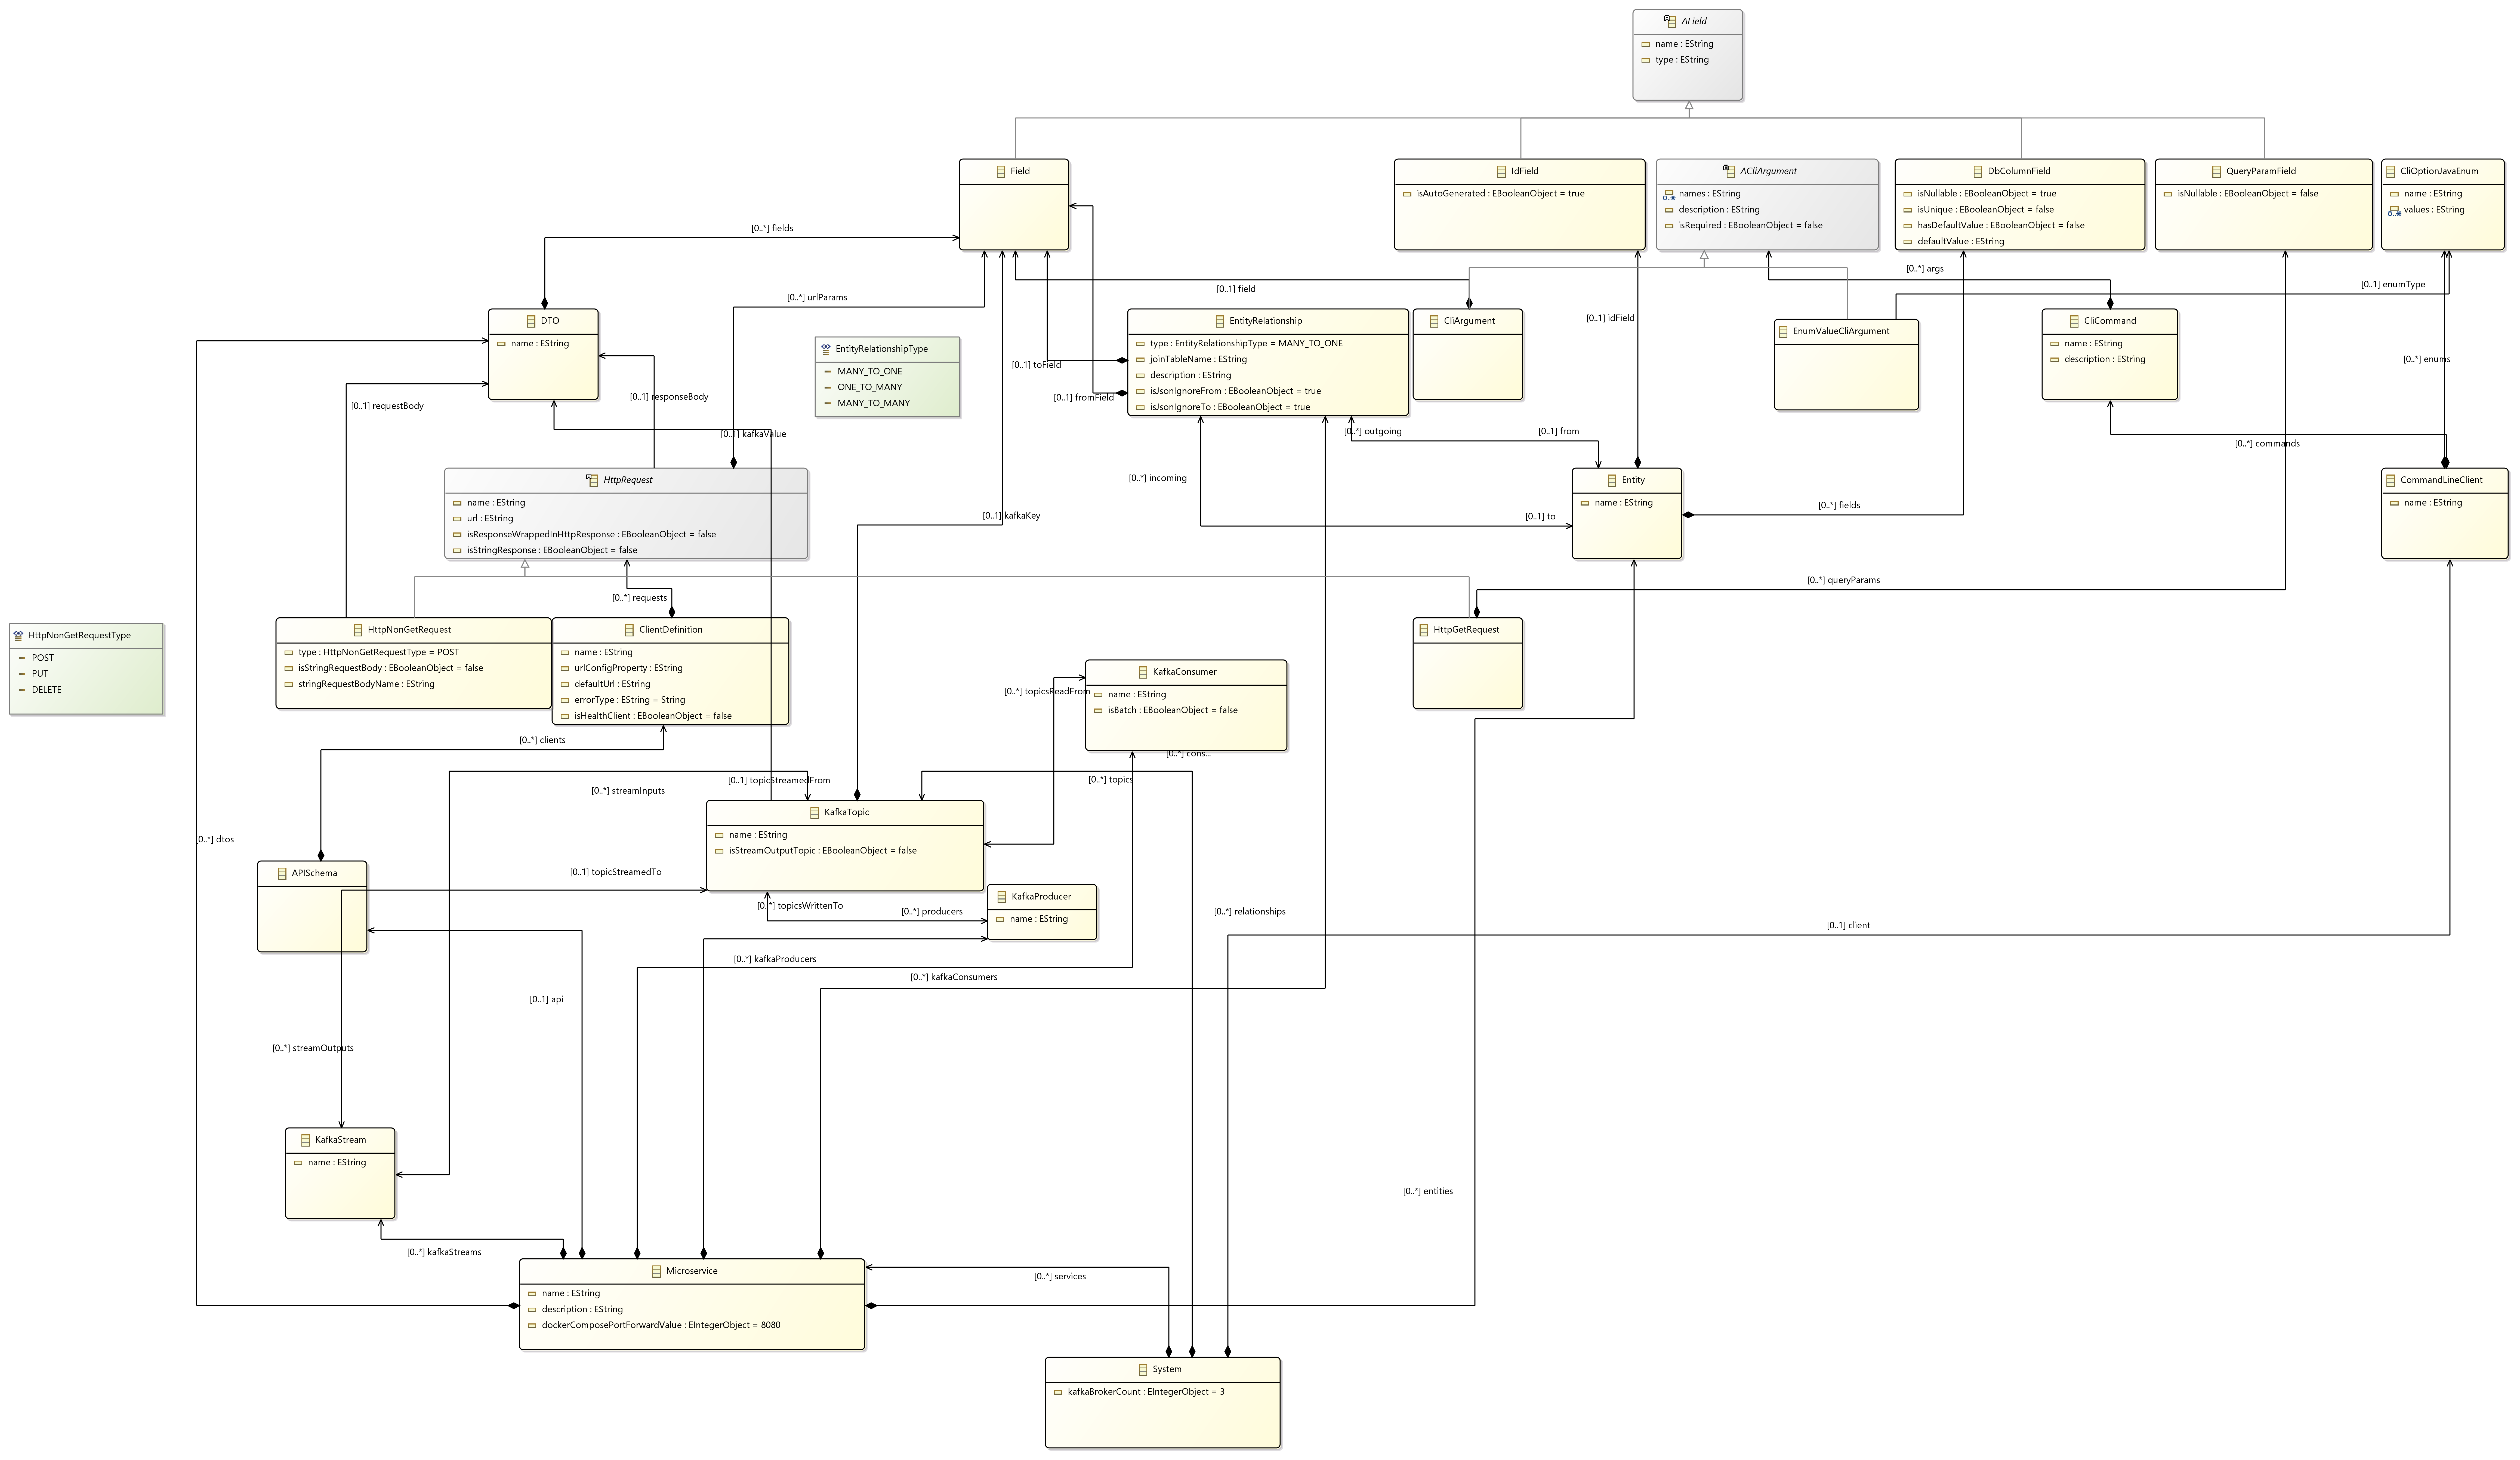
\includegraphics[width=\textwidth]{metamodel-class-diagram}
        \caption{Metamodel class diagram}
        \label{fig:metamodelDiagram}
    \end{figure}

    The metamodel in figure \ref{fig:metamodelDiagram} describes a multi-component system with a command line interface.
    Since the model's main use will be the generation of code implementing parts of such a system, the metamodel includes the Afield class, representing a variable in some programming language.
    Instances inheriting this class will have at least a name and a type, both strings.
    The root class of the model is the System class, which contains the top-level, general information about the system, such as the number of Kafka brokers, the message exchange topics and its components.
    The components of a System are one or more instances of the Microservice class and exactly one instance of the CommandLineClient class.
    The CommandLineClient class contains information about the available commands as well as a separate field, ``enums'' which contains one or more enums storing the possible options for certain args.
    Each command has attributes for its name and description as well as zero or many args, each of which is defined by a name, type and the variable the argument maps to.
    The Microservice class aims to define the domain logic of a component of the system.
    Therefore, it includes information about the following:
    \begin{itemize}
        \item	The name of the microservice
        \item	The entities in its domain
        \begin{itemize}
            \item Each entity has exactly one ID field
            \item Each entity has zero or many ``Column fields'', which extend the Afield class with information such as whether the field is nullable or unique in the database.
            \item Entities contain references to incoming and outgoing relationships
        \end{itemize}
        \item	Message exchange components i.e. Kafka consumers, producers, and streams
        \begin{itemize}
            \item Kafka producers contain references to topics they write to
            \item Kafka consumers contain references to topics they read from as well as whether they process their messages in batches or not
            \item Kafka streams contain references to both input and output topics
        \end{itemize}
        \item	The external facing API of the microservice
        \begin{itemize}
        \item The API is represented by an instance of the APISchema class
        \item This object contains information about each of the controllers present in the microservice, which in turn contain information about the available endpoints, their URL's, any URL parameters, query parameters, as well as the response object type
        \end{itemize}
        \item	The DTOs used both in HTTP communication and message exchange
        \item	The number of the port on which the service is expected to be available in a container orchestration scenario (e.g. docker compose)
        \item	Relationships between entities
        \begin{itemize}
        \item Each relationship object contains information about the source and target entity, as well as the name of the fields storing this information in the code implementation (e.g. the ``viewers'' and ``viewedVideos'' fields on video and user entities respectively)
        \item The type of relationship is also stored here (many to many, one to many etc.)
        \item Note:  while it might seem that the ONE\_TO\_MANY and MANY\_TO\_ONE relationship types are duplicates, this is an adaptation to the specifics of micronaut.
        This adaptation was applied in section 2.2.4, where only the ``target'' entity's field contained the ``mappedBy'' annotation, allowing developers to customize which side of the relationship can accept edits when writing Java code.
        \end{itemize}
        While the model aims to be as general as possible, it still makes some assumptions about the design of the system:
        \item	The system shall have a single CLI client (or at least, a single CLI project)
        \begin{itemize}
        \item While a system with a greater number of components and/or developer teams working on it may benefit from having several distinct projects for the command line clients, the increased amount of required setup (e.g. maintaining several nested java projects, repeated build scripts) was deemed not worth it.
        \end{itemize}
        \item	The system shall use Apache Kafka for its message exchange
        \begin{itemize}
        \item Different messaging systems use different terminology for its components (e.g. topics vs event streams).
        \end{itemize}
        Since Kafka is the chosen system for this project, limiting the metamodel to only Kafka concepts and terminology was deemed a worthy tradeoff over maximizing generalizability.
        \item	The users of the concrete graphical synthax will be responsible for providing correct types when adding typed values (e.g. column fields for entities)
        \begin{itemize}
        \item Since it is impossible to predict the exact dependencies or types of each field, the metamodel leaves it up to the developer to provide valid types for their programming language of choice (e.g. Java for the current project)
        \end{itemize}
        The following design choices have been considered but rejected in the final version:
        \item	Not having separate types for GET and non-GET HTTP requests
        \begin{itemize}
        \item This was dismissed as it made the model validation rules less clear, particularly with request bodies, as these are typically not used for GET requests
        \end{itemize}
        \item	Linking CLI commands and HTTP requests
        \begin{itemize}
        \item This was dismissed as while it would allow for a clearer link between microservice functionality and the CLI interface, it could potentially limit the functionality of the client, e.g. when requesting information from one microservice and using the response data to make another request
            \end{itemize}
    \end{itemize}
    \pagebreak
    \subsection{Graphical concrete synthax}
    TODO
    \pagebreak
    \subsection{Model validation}
    Table \ref{tab:evlTable} contains the list of EVL validations that was applied to the model.
    Highlighted rows are warnings (critiques) while the rest are errors (constraints).
    Critiques that do not directly affect the submission criteria have been omitted for brevity.

    \begin{table}[h]
        \centering
        \begin{tabular}{|p{0.21\linewidth}|p{0.4\linewidth}|p{0.39\linewidth}|}
            \toprule
            \textbf{Context} & \textbf{Name} & \textbf{Description} \\
            \midrule
            \rowcolor{lightgray}
            KafkaTopic & shouldHaveAtLeastOneConsumer &  \\
            \hline
            \rowcolor{lightgray}
            KafkaTopic & shouldHaveAtLeastOneProducer &  \\
            \hline
            KafkaTopic & mustHaveKafkaKeyField &  \\
            \hline
            KafkaTopic & mustHaveValueDTO &  \\
            \hline
            Entity & mustHaveIdField & Error if entity does not have an @ID annotated field \\
            \hline
            EntityRelationship & mustHaveToEntity &  \\
            \hline
            EntityRelationship & mustHaveFromEntity &  \\
            \hline
            EntityRelationship & mustHaveToField & Entities must have a java field for incoming/outgoing relationships \\
            \hline
            EntityRelationship & mustHaveFromField & \\
            \hline
            System & mustHaveAtLeastOneMicroservice &  \\
            \hline
            System & \hspace{0pt}microservicesMustNotExposeConflictingPorts & Error if several microservices are exposing the same port in docker compose \\
            \hline
            Microservice & nameMustNotContainSpaces &  \\
            \hline
            Microservice & mustHaveDifferentJoinTablesForMultipleMany\-ToManyRelationships & Error if there are several many to many relationships using the same join table \\
            \hline
            APISchema & mustHaveOneHealthEndpoint & Every microservice must have a health client. \\
            \hline
            HttpRequest & \hspace{0pt}mustNotHaveAResponseBodyDTOIfStringResponse &  \\
            \hline
            HttpRequest & mustHaveAFieldForEveryURLParameter & Error if no java value exists for any URL parameter \\
            \hline
            HttpRequest & mustNotHaveBackToBackURLParameters & Error if URL has several parameters without a slash e.g. /\{id\}\{name\} \\
            \hline
            HttpRequest & mustHaveAURLParameterForEveryField & Error if no URL parameter exists for any of the java values in the request method \\
            \hline
            HttpNonGetRequest &\hspace{0pt}mustNotHaveARequestBodyDTOIfStringRequestBody &  \\
            \hline
            HttpNonGetRequest & mustHaveType & Non - GET requests must specify a type - POST, PUT etc. \\
            \hline
            ClientDefinition & mustHaveAtLeastOneRequest &  \\
            \hline
            ClientDefinition & healthClientMustHaveOneHealthGetEndpoint &  \\
            \hline
            Afield & typeMustStartWithUpperCase & Type must be a java type i.e. start with uppercase letter \\
            \hline
            CommandLineClient & mustHaveAtLeastOneCommand &  \\
            \hline
            CLICommand &\hspace{0pt}mustNotHaveDifferentArgumentsWithSameName & Error if several CLI args for a command attempt to use the same name \\
            \hline
            EnumValueCliArgument & mustHaveDefinedEnum & Error if doesn't reference an existing enum \\
            \hline
            CliArgument & mustHaveDefinedField &  \\
            \bottomrule
        \end{tabular}
        \caption{EVL validation rules}
        \label{tab:evlTable}
    \end{table}

    \pagebreak
    \subsection{Model-to-text transformation}
    \subsubsection{M2T code organisation}
    The model was used to generate a significant amount of code for the microservices.
    The resulting code was written to several places, depending on the functionality it provided:
    \begin{itemize}
\item	Microservice-specific code, such as generated entities, Kafka consumers and the interfaces defining Kafka producers and streams, were written to each microservice's folder.
In order to separate generated and manually written code, the output directory was placed inside the``build''folder and marked as an additional source set in each gradle build file.
This allowed the generated code to be easily deleted (e.g. by running gradle clean), placed it``out of sight''of the developer and made it clear that the code is not to be edited manually.
\item	Code that related to data transfer or was otherwise needed by each microservice was placed in a separate project, named``generated-shared''.
This code included the following:
\begin{itemize}
    \item	Http clients
    \item	Interfaces defining the behaviour of Http controllers
    \item	Kafka topic names (as static String variables)
    \item	DTO definitions (both for HTTP response types and Kafka messages)
\end{itemize}
To include this code into another microservice, the``generated-shared''project could simply be added as a dependency via the build.gradle file.
\item	CLI client specific code, such as argument option enums and scaffolds for implementing the CLI commands was written to the``client''project using the same approach as when writing code to the microservices' directories.
\item	The generated part of the docker compose cluster was written to the top level in the``microservices''directory.
\end{itemize}
While writing code to several directories at once slightly increased the complexity of the EGX orchestration, it provided several key benefits: first, it allowed bean classes to be generated for one microservice without polluting the context of any other microservice that needs to share some code with it.
For example, by not sharing any @Entity beans, each microservice's domain would be strictly limited to the entities it is concerned with.
Second, for classes that do not affect the micronaut app such as simple DTO definitions or re-used HTTP clients, the shared project became a convenient way to reuse code and avoid excessive boilerplate.

    \subsubsection{M2T transformation implementation details}
    This section will outline the approaches taken to convert the model into java code for the microservices.
    \begin{itemize}
\item	Kafka consumers and streams were transformed to java interfaces.
Since the logic of handling an incoming message is too complex to be captured in a model, the implementation was left to the developer.
It should be noted that while the @Topic annotation is able to be inherited, the @KafkaListener annotation is not.
Therefore a choice was made to not annotate the generated functions with @Topic, as having all the annotations in a single place (the interface implementation code) improves code readability for developers.
\item	Kafka producers, only requiring an interface, were fully implemented in the generated code.
The topic names as well as key and value types were determined from the``topicsWrittenTo''references of the KafkaProducer class.
\item	DTO classes were transformed into java record classes, annotated with @Serdeable.
While record classes are only available to java versions 17 and above, it matched the entire project's java version, which made this design choice an appropriate one for reducing the quantity of the written code as well as the need to write getters and setters for the newly created objects.
\item	For each``ClientDefinition''class, 2 java objects have been created: an HTTP client interface, annotated with request types and client URL (with both the matching config property and a default value) and an interface that only specified the name of each request, its return type and any parameters.
This allowed the generated code to contain a fully ready to inject client as well as a scaffold for implementing a controller.
Similarly to Kafka consumers, some annotations were inherited (e.g. request types) while others were not (@Controller).
Therefore, it was up to the developer to add all the annotations, e.g. by matching the generated client interface.
This, while adding some effort, increased the readability and``self-documentation''of the code.
\item	For the CLI commands, abstract classes, named after the command name with the prefix``A''were generated.
Each class contained the @Command annotation (which can be inherited) as well as the definition for each argument variable, which were determined from the``args''property of the CliCommand class.
The command description, standard help options and argument descriptions were also generated, with the latter also describing possible options for enum arguments.
The variables for the argument were made``protected''so that classes that extend the abstract class can make use of it.
It should be noted that while the contents (i.e. description, standard help options etc.) of the @Command annotation are inherited, the annotation itself is not.
This means that in order to satisfy the compiler, the manually written commands need to be annotated with @Command, which only has to include the command name.
While this approach goes slightly against that of the HTTP controllers, it saves the developer from having to manually copy over argument descriptions and names, making it a worthwhile departure from the rest of the generated code.
\item	The docker compose file was generated from the root System class and included the images of each microservice with a separate database container for each one (as described in 2.1.1).
The generated docker compose did not include sensitive data like database passwords in order to mimic a production-like environment and to not give the model generation templates access to secrets.
\item	Entity classes were also fully generated.
Entity relationships were constructed by checking the``toField''and``fromField''on``incoming''and``outgoing''relationships respectively.
As described in 2.2.1, only the``incoming''transitions contained the ``mappedBy'' micronaut field, which allowed the generated code to match the intended use case e.g. when the desired way of adding a user to a video is by changing the user entity rather than the video entity.
Convenience methods for modifying entities were written, as needed, in the``utils''package of the corresponding microservice.
Overall, the generated code allowed for a significant saving in effort when writing the microservices.
The only things up to the user were making sure that all microservices' projects are created (with the right source set added), writing the controller behaviour, the repositories, the Kafka consumers (and streams) and the behaviour of the CLI commands.
While this is still a significant undertaking, not needing to write the mostly boilerplate code of the remaining parts of the system allows the developer to focus purely on adhering to the requirements and making sure that the business logic is executed correctly.
\end{itemize}
    \pagebreak
    \section{References}
    TODO TODO TODO



\end{document}
